\part{集群方案篇}

本章介绍几种高可用的解决方案。

\chapter{集群基础知识}

\section{集群概述}

集群是一组协同工作的服务实体,用以提供比单一服务实体更具扩展性和可用性
的服务平台。

在客户端看来,一个集群就是一个完整不可细分的实体,但事实上一个集群实体
是由完成不同任务的服务节点个体所组成的。

集群实体的可扩展性是指,在集群运行中新的服务节点可以动态的加入集群实体
从而提升集群实体的综合性能。

集群实体的高可用性是指,集群实体通过其内部的服务节点的冗余使客户端免于
OUT OF SERVICE错误。简单的说,在集群中同一服务可以由多个服务节点提供,
当部分服务节点失效后,其他服务节点可以接管服务。

集群实体地址是指客户端访问集群实体获得服务资源的唯一入口地址。

负载均衡是指集群中的分发设备(服务)将用户的请求任务比较均衡(不是平均)
分发到集群实体中的服务节点计算、存储和网络资源中。一般我们将提供负载均
衡分发的设备叫做负载均衡器。负载均衡器一般具备如下三个功能:

\begin{enumerate}[itemsep=0pt,parsep=0pt]
\item 维护集群地址
\item 负责管理各个服务节点的加入和退出
\item 集群地址向内部服务节点地址的转换
\end{enumerate}

错误恢复是指集群中某个节点或某些服务节点(设备)不能正常工作(或提供服
  务),其他类似服务节点(设备)可以资源透明和持续的完成原有任务。具备
错误恢复能力是集群实体高可用性的必要条件。

负载均衡和错误恢复都需要集群实体中各个服务节点中有执行同一任务的资源存
在,而且对于同一任务的各个资源来说,执行任务所学的信息视图必须一致。

\section{集群类型}

多台同构或异构的计算机用某种方式连接起来协同完成特定的任务就构成了集群
系统,目前Linux下的集群主要有三种类型:

\begin{enumerate}[itemsep=0pt,parsep=0pt]
\item HA(High Availability)
\item LB(Load Balancing)
\item HPC(High Performance Computing)
\end{enumerate}

\chapter{Keepalived}
\label{chap:keepalived}

\section{Keepalived简介}

KeepAlived起初是专为LVS设计的,专门用来监控LVS集群系统中各个服务节点的
状态,后来又加入了VRRP的功能,因此,除了配合LVS服务外,也可以作为其他服
务(如Nginx,HAProxy等)的高可用软件。VRRP是Virtual Router Redundancy
Protocol(虚拟路由冗余协议)的缩写,VRRP出现的目的就是为了解决静态路由
出现的单点故障问题,它能够保证网络的不间断、稳定地运行。所
以,KeepAlived一方面具有LVS cluster nodes healthcheck功能,另一方面也具
有LVS directors failover功能。

\section{Keepalived安装部署}

\subsection{环境准备}

演示环境为CentOS6.5 64位系统,机器列表如下:

\begin{table}[!htbp]
  \centering
  \caption{KeepAlived演示环境机器列表}
  \begin{tabular}{|l|l|r|}
    \hline
    主机名  & IP地址 & 角色 \\
    \hline
    lb01.lavenliu.com & 192.168.20.150 & KeepAlived(主) \\
    \hline
    lb02.lavenliu.com & 192.168.20.151 & KeepAlived(备) \\
    \hline
  \end{tabular}
\end{table}

\subsection{开始安装}

\begin{verbatim}
yum install -y keepalived
\end{verbatim}

\subsection{Keepalived配置介绍}

\section{运行服务与故障模拟}


\chapter{LVS+Keepalived负载均衡集群}

LVS(Linux Virtual Server) is a cluster of servers 

The Linux Virtual Server can be used to build scalable network
services based on a cluster of two or more nodes. The active node of
the cluster redirects service requests to a collection of server hosts
that will actually perform the services. Supported features include
two protocols (TCP and UDP), three packet-forwarding methods (NAT,
tunneling, and direct routing), and eight load balancing algorithms
(round robin, weighted round robin, least-connection, weighted
least-connection, locality-based least-connection, locality-based
least-connection with replication, destination-hashing, and
source-hashing).

LVS: ipvsadm/ipvs

When a new connection is requested from a client to a service provided
by the LVS (e.g. httpd), the director will choose a realserver from
the client.

From then, all packets from the client will go through the director to
that particular realserver.

The association between the client and the realserver will last for
only the life of the tcp connection (or udp exchange).

For the next tcp connection, the director will choose a new realserver
(which may or may not be the same as the first realserver).

Thus a web browser connecting to a LVS serving a webpage consisting of
several hits (images, html page), may get each hit from a separate
realserver.

LVS IP Address Name Conventions

Virtual IP (VIP) address: The IP address the Director uses to offer
services to client computers

Real IP (RIP) address: The IP address used on the cluster nodes

Director's IP (DIP) address: The IP address the Director uses to
connect to the D/RIP network

Client computer's IP (CIP) address: The IP address assigned to a
client computer that it uses as a source IP address for requests sent
to the cluster

\begin{quote}
  Basic Properties of LVS-NAT 

1. The cluster nodes need to be on the
same network (VLAN or subnet) as the Director.
集群节点必须与调度器在同一个网络中


2. The RIP addresses of the cluster nodes are normally private,
non-routable IP addresses used only for intracluster communication.
RIP通常是私有地址,仅用于各集群节点间的通信

3. director位于client与real server之间,并负责处理进出的所有通信

4. realserver必须将网关指向DIP

5. 支持端口映射

6. real server可以使用任何操作系统

7. 较大规模应用场景中,director易成为系统瓶颈
\end{quote}

\begin{quote}
  1. 集群节点跟director必须在同一物理网络中

  2. RIP可以使用公网地址,实现便捷的远程管理和监控

  3. director仅负责处理入站请求,响应报文则由real server直接发往客户端

  4. real server不能讲网关指向DIP

  5. 不支持端口映射

  real server必须能够隐藏VIP
\end{quote}

\begin{quote}
  TUN:
  1. 集群节点可以跨越Internet
  2. RIP必须是公网地址
  3. Director仅处理入站请求,响应报文则由real server直接发往客户端
  4. real server网关不能指向director
  5. 只有支持隧道功能的os才能用于real server
  6. 不支持端口映射
\end{quote}

\section{LVS调度算法}

Director在接收到来自于Client的请求时,会基于"schedule"从RealServer中选
择一个响应给Client。ipvs支持以下调度算法:

\begin{enumerate}[itemsep=0pt,parsep=0pt]
\item 轮询(round robin, rr),加权轮询(Weighted round robin, wrr)

  新的连接请求被轮流分配至各RealServer;算法的优点是其简洁性,它无需记
  录当前所有连接的状态,所以它是一种无状态调度。轮叫调度算法假设所有服
  务器处理性能均相同,不管服务器的当前连接数和响应速度。该算法相对简单,
  不适用于服务器组中处理性能不一的情况,而且当请求服务时间变化比较大时,
  轮叫调度算法容易导致服务器间的负载不平衡。

\item 最少连接(least connected, lc), 加权最少连接(weighted least
  connection, wlc)

  新的连接请求将被分配至当前连接数最少的RealServer;最小连接调度是一种
  动态调度算法,它通过服务器当前所活跃的连接数来估计服务器的负载情况。
  调度器需要记录各个服务器已建立连接的数目,当一个请求被调度到某台服务
  器,其连接数加1;当连接中止或超时,其连接数减一。

\item 基于局部性的最少链接调度(Locality-Based Least Connections
  Scheduling,lblc)

  针对请求报文的目标IP地址的负载均衡调度,目前主要用于Cache集群系统,因
  为在Cache集群中客户请求报文的目标IP地址是变化的。这里假设任何后端服务
  器都可以处理任一请求,算法的设计目标是在服务器的负载基本平衡情况下,
  将相同目标IP地址的请求调度到同一台服务器,来提高各台服务器的访问局部
  性和主存Cache命中率,从而整个集群系统的处理能力。LBLC调度算法先根据请
  求的目标IP地址找出该目标IP地址最近使用的服务器,若该服务器是可用的且
  没有超载,将请求发送到该服务器;若服务器不存在,或者该服务器超载且有
  服务器处于其一半的工作负载,则用“最少链接”的原则选出一个可用的服务
  器,将请求发送到该服务器。

\item 带复制的基于局部性最少链接调度(Locality-Based Least Connections
  with Replication Scheduling,lblcr)

  也是针对目标IP地址的负载均衡,目前主要用于Cache集群系统。它与LBLC算法
  的不同之处是它要维护从一个目标IP地址到一组服务器的映射,而 LBLC算法维
  护从一个目标IP地址到一台服务器的映射。对于一个“热门”站点的服务请求,
  一台Cache 服务器可能会忙不过来处理这些请求。这时,LBLC调度算法会从所
  有的Cache服务器中按“最小连接”原则选出一台Cache服务器,映射该“热
  门”站点到这台Cache服务器,很快这台Cache服务器也会超载,就会重复上述
  过程选出新的Cache服务器。这样,可能会导致该“热门”站点的映像会出现在
  所有的Cache服务器上,降低了Cache服务器的使用效率。LBLCR调度算法将“热
  门”站点映射到一组Cache服务器(服务器集合),当该“热门”站点的请求负
  载增加时,会增加集合里的Cache服务器,来处理不断增长的负载;当该“热
  门”站点的请求负载降低时,会减少集合里的Cache服务器数目。这样,该“热
  门”站点的映像不太可能出现在所有的Cache服务器上,从而提供Cache集群系
  统的使用效率。LBLCR算法先根据请求的目标IP地址找出该目标IP地址对应的服
  务器组;按“最小连接”原则从该服务器组中选出一台服务器,若服务器没有
  超载,将请求发送到该服务器;若服务器超载;则按“最小连接”原则从整个
  集群中选出一台服务器,将该服务器加入到服务器组中,将请求发送到该服务
  器。同时,当该服务器组有一段时间没有被修改,将最忙的服务器从服务器组
  中删除,以降低复制的程度。

\item 目标地址散列调度(Destination Hashing,dh)

  算法也是针对目标IP地址的负载均衡,但它是一种静态映射算法,通过一个散
  列(Hash)函数将一个目标IP地址映射到一台服务器。目标地址散列调度算法
  先根据请求的目标IP地址,作为散列键(Hash Key)从静态分配的散列表找出
  对应的服务器,若该服务器是可用的且未超载,将请求发送到该服务器,否则
  返回空。

\item 源地址散列调度(Source Hashing,sh)

  算法正好与目标地址散列调度算法相反,它根据请求的源IP地址,作为散列键
  (Hash Key)从静态分配的散列表找出对应的服务器,若该服务器是可用的且
  未超载,将请求发送到该服务器,否则返回空。它采用的散列函数与目标地址
  散列调度算法的相同。除了将请求的目标IP地址换成请求的源IP地址外,它的
  算法流程与目标地址散列调度算法的基本相似。在实际应用中,源地址散列调
  度和目标地址散列调度可以结合使用在防火墙集群中,它们可以保证整个系统
  的唯一出入口。
\end{enumerate}


基于DNS的负载均衡方案性能可能会出现问题。DNS的记录会缓存。

rsync基于文件的同步,效率低。

drbd磁盘镜像,让两个计算机的两块磁盘做镜像,基于块级别的同步,效率高。

\section{安装LVS}
\label{installLVS}

\subsection{环境准备}
\label{sec:lvsEnvPrepare}



\chapter{Heartbeat高可用集群}

Heartbeat提供了诸多集群基础架构服务,比如集群之间的消息传递、节点成员
身份、IP地址分配和迁移,以及服务的开启和停止。Heartbeat可以用来为
Apache、Samba和Squid等企业应用系统构建几乎任何一种高可用性的集群。此外,
它可以结合负载均衡软件使用,那样入站请求就可以由所有集群节点来分担。

本文中的示例集群将由2台运行Heartbeat的服务器组成。我们测试故障切换机
制的方法是,手动关闭服务器,检查它们服务的网站是不是仍然可用。下面是我
们的测试拓扑结构:

\begin{figure}[!htbp]
  \centering
  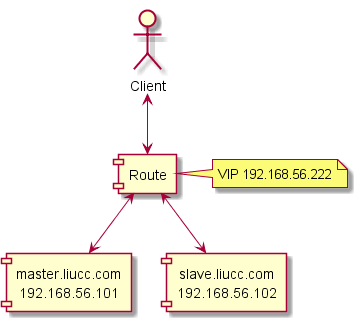
\includegraphics[width=0.5\textwidth]{img/heartbeat.png}
  \caption{heartbeat实验拓扑}
\end{figure}

映射服务所用的IP地址需要一直能够访问得到。通常,Heartbeat会为你将指定
的IP地址分配给主服务器上的虚拟网络接口卡。如果主服务器出现了故障,集群
会自动将IP地址切换到另一台可用服务器上的虚拟网卡。如果主服务器恢复正常
运行,它会再次将IP地址切换回到主服务器。由于具有迁移属性,这个IP地址被
称为“浮动”地址。

\section{安装Heartbeat}

在所有服务器上安装软件包

想组建集群,首先要使用yum,在每一个节点上安装必要的软件包:

\begin{verbatim}
yum install PyXML cluster-glue cluster-glue-libs resource-agents
\end{verbatim}

下一步,下载和安装官方CentOS软件库里面没有的两个Heartbeat RPM文件。

另外,你可以将EPEL软件库添加到源文件,并使用yum进行安装。

Heartbeat会管理Apache的httpd服务的开启和停止,所以停止Apache,并禁止它自动开启:

\begin{verbatim}
service httpd stop
chkconfig httpd off
\end{verbatim}

设置主机名称

现在设置服务器的主机名称,为此编辑每个系统上的/etc/sysconfig/network,并更改HOSTNAME这一行:

HOSTNAME=xxxxx.liucc.com 新的主机名称会在服务器下一次启动时激活。
你可以使用hostname命令立即激活它,不需要重启服务器:

hostname xxxxx.liucc.com 你可以在每一台服务器上运行uname -n,以此证实主机名称已正确设置好。

\section{配置Heartbeat}

想配置Heartbeat,首先要将其默认配置文件从/usr拷贝到/etc/ha.d/:

\begin{verbatim}
cp /usr/share/doc/heartbeat-3.0.4/authkeys /etc/ha.d/
cp /usr/share/doc/heartbeat-3.0.4/ha.cf /etc/ha.d/
cp /usr/share/doc/heartbeat-3.0.4/haresources /etc/ha.d/
\end{verbatim}

然后,你还得改动全部集群节点上的所有三个文件,以便与你的需求相匹配。

authkeys文件含有集群节点彼此联系时所使用的预共享密码。集群里面的每个
Heartbeat消息都含有该密码,节点只处理拥有正确密码的那些消息。Heartbeat
支持SHA1密码和MD5密码。在authkeys文件中,下列指令将验证方法设置为SHA1,
并且定义了所使用的密码:

\begin{verbatim}
auth 2
2 sha1 pre-shared-password
\end{verbatim}

保存该文件,然后使用命令

\begin{verbatim}
chmod 600 /etc/ha.d/authkeys
\end{verbatim}

为该文件授予只有root用户可以读写的权限。

下一步,在ha.cf文件中,定义计时器、集群节点、消息传递机制、第4层端口及其他设置:

\begin{verbatim}
## 日志##
logfile /var/log/ha-log
logfacility local0hea
## 计时器##
## 所有计时器设成以秒为单位。如果你需要以毫秒为单位设置时间,就使用‘ms’。##
## heartbeat间隔时间##
keepalive 2

## 超过这个时间后,节点被认为已停滞##
deadtime 15
## 一些服务器花更长的时间来启动。该计时器定义了证实服务器宕机之前所等待的额外时间。##
## 该计时器的建议时间是停滞计时器的至少一倍。##
initdead 120
## 消息传递参数##
udpport 694
bcast eth0
## 你还可以使用多播或单播##
## 节点定义##
## 确保主机名称符合uname -n ##
node master.liucc.com
node slave.liucc.com
\end{verbatim}

最后,文件haresources含有Heartbeat认为是主节点的那台服务器的主机名称,
另外还含有浮动IP地址。该文件在所有服务器上都一模一样,这点很重要。只要
主节点在正常运行,它就服务所有请求;Heartbeat停止其他所有节点上的高可
用性服务。Heartbeat检测到该主节点停机运行后,它会在集群中的下一个可用
节点上自动开启服务。主节点恢复正常运行后,Heartbeat会让它再次接手任务,
服务所有请求。最后,该文件含有负责高可用性服务的脚本的名称:这里是
httpd。其他可能出现的值有squid、smb、nmb或postfix,映射到通常位于
/etc/init.d/目录中的服务启动脚本的名称。

在haresources中,定义master.liucc.com.com为主服务器,定义
192.168.56.222为浮动IP地址,定义 httpd为高可用性服务。你不需要创建任何
接口,也不需要为任何接口手动分配浮动IP地址,Heartbeat为我们处理这项任
务:

\begin{verbatim}
master.liucc.com 192.168.56.222 httpd
\end{verbatim}

每一台服务器上的配置文件准备就绪后,开启Heartbeat服务,并将它添加到系
统启动项:

\begin{verbatim}
service heartebeat start
chkconfig heartbeat on
\end{verbatim}

这时,可以查看一下master节点上的IP地址信息,

\begin{verbatim}
[root@master ~]# ifconfig 
eth0      Link encap:Ethernet  HWaddr 08:00:27:4D:65:37  
          inet addr:192.168.56.101  Bcast:192.168.56.255  Mask:255.255.255.0
          inet6 addr: fe80::a00:27ff:fe4d:6537/64 Scope:Link
          UP BROADCAST RUNNING MULTICAST  MTU:1500  Metric:1
          RX packets:13825 errors:0 dropped:0 overruns:0 frame:0
          TX packets:10376 errors:0 dropped:0 overruns:0 carrier:0
          collisions:0 txqueuelen:1000 
          RX bytes:3095677 (2.9 MiB)  TX bytes:2253820 (2.1 MiB)

eth0:0    Link encap:Ethernet  HWaddr 08:00:27:4D:65:37  
          inet addr:192.168.56.222  Bcast:192.168.56.255  Mask:255.255.255.0
          UP BROADCAST RUNNING MULTICAST  MTU:1500  Metric:1

eth1      Link encap:Ethernet  HWaddr 08:00:27:BC:A6:E2  
          inet addr:192.168.56.201  Bcast:192.168.56.255  Mask:255.255.255.0
          inet6 addr: fe80::a00:27ff:febc:a6e2/64 Scope:Link
          UP BROADCAST RUNNING MULTICAST  MTU:1500  Metric:1
          RX packets:21609 errors:0 dropped:0 overruns:0 frame:0
          TX packets:61 errors:0 dropped:0 overruns:0 carrier:0
          collisions:0 txqueuelen:1000 
          RX bytes:4926438 (4.6 MiB)  TX bytes:6922 (6.7 KiB)

lo        Link encap:Local Loopback  
          inet addr:127.0.0.1  Mask:255.0.0.0
          inet6 addr: ::1/128 Scope:Host
          UP LOOPBACK RUNNING  MTU:16436  Metric:1
          RX packets:2696 errors:0 dropped:0 overruns:0 frame:0
          TX packets:2696 errors:0 dropped:0 overruns:0 carrier:0
          collisions:0 txqueuelen:0 
          RX bytes:5452373 (5.1 MiB)  TX bytes:5452373 (5.1 MiB)
\end{verbatim}

你可以借助命令tailf /var/log/ha-log,密切关注Heartbeat日志。

Heartbeat可用于多项服务。比如说,haresources中的下列指令将让Heartbeat
同时管理Apache服务和Samba服务:

master.liucc.com 192.168.56.222 httpd smb nmb 不过,除非你还在运行
Pacemaker之类的集群资源管理器(CRM),否则我不建议使用Heartbeat在单一
集群中提供多项服务。要是没有Pacemaker,Heartbeat使用IP地址监测第3层中
的集群节点。只要IP地址可以访问得到,Heartbeat无视服务在服务器节点上可
能遇到的任何崩溃或困难。

\section{测试}

一旦Heartbeat设置并运行起来,不妨对它测试一下。在所有三台服务器上创建
单独的index.html文件,那样你就能看清哪台服务器在服务页面。浏览到
192.168.56.222,如果你设置好了DNS,也可以浏览到相应域名。页面应该会从
master.liucc.com.com加载,你可以查看服务器1中的Apache日志文件来核实这一
点。试着刷新页面,证实该页面是否每次都从同一台服务器加载。

关闭主节点后,主节点产生的日志信息,

\begin{verbatim}
Apr 14 11:43:48 master.liucc.com heartbeat: [13928]: info: Heartbeat shutdown in progress. (13928)
Apr 14 11:43:48 master.liucc.com heartbeat: [14300]: info: Giving up all HA resources.
ResourceManager[14313]:	2015/04/14_11:43:48 info: Releasing resource group: master.liucc.com 192.168.56.222 httpd
ResourceManager[14313]:	2015/04/14_11:43:48 info: Running /etc/init.d/httpd  stop
ResourceManager[14313]:	2015/04/14_11:43:48 info: Running /etc/ha.d/resource.d/IPaddr 192.168.56.222 stop
IPaddr[14386]:	2015/04/14_11:43:48 INFO: ifconfig eth0:0 down
IPaddr[14372]:	2015/04/14_11:43:48 INFO:  Success
Apr 14 11:43:48 master.liucc.com heartbeat: [14300]: info: All HA resources relinquished.
Apr 14 11:43:49 master.liucc.com heartbeat: [13928]: WARN: 1 lost packet(s) for [slave.liucc.com] [36:38]
Apr 14 11:43:49 master.liucc.com heartbeat: [13928]: info: No pkts missing from slave.liucc.com!
Apr 14 11:43:50 master.liucc.com heartbeat: [13928]: info: killing HBFIFO process 13930 with signal 15
Apr 14 11:43:50 master.liucc.com heartbeat: [13928]: info: killing HBWRITE process 13931 with signal 15
Apr 14 11:43:50 master.liucc.com heartbeat: [13928]: info: killing HBREAD process 13932 with signal 15
Apr 14 11:43:50 master.liucc.com heartbeat: [13928]: info: Core process 13932 exited. 3 remaining
Apr 14 11:43:50 master.liucc.com heartbeat: [13928]: info: Core process 13931 exited. 2 remaining
Apr 14 11:43:50 master.liucc.com heartbeat: [13928]: info: Core process 13930 exited. 1 remaining
Apr 14 11:43:50 master.liucc.com heartbeat: [13928]: info: master.liucc.com Heartbeat shutdown complete.
\end{verbatim}

此时,备节点上的日志信息为:

\begin{verbatim}
ResourceManager[13103]:	2015/04/14_11:43:49 info: Acquiring resource group: master.liucc.com 192.168.56.222 httpd
IPaddr[13131]:	2015/04/14_11:43:49 INFO:  Resource is stopped
ResourceManager[13103]:	2015/04/14_11:43:49 info: Running /etc/ha.d/resource.d/IPaddr 192.168.56.222 start
IPaddr[13194]:	2015/04/14_11:43:49 INFO: Using calculated nic for 192.168.56.222: eth0
IPaddr[13194]:	2015/04/14_11:43:49 INFO: Using calculated netmask for 192.168.56.222: 255.255.255.0
IPaddr[13194]:	2015/04/14_11:43:49 INFO: eval ifconfig eth0:0 192.168.56.222 netmask 255.255.255.0 broadcast 192.168.56.255
IPaddr[13180]:	2015/04/14_11:43:49 INFO:  Success
ResourceManager[13103]:	2015/04/14_11:43:49 info: Running /etc/init.d/httpd  start
mach_down[13076]:	2015/04/14_11:43:49 info: /usr/share/heartbeat/mach_down: nice_failback: foreign resources acquired
mach_down[13076]:	2015/04/14_11:43:49 info: mach_down takeover complete for node master.liucc.com.
Apr 14 11:43:49 slave.liucc.com heartbeat: [12969]: info: mach_down takeover complete.
Apr 14 11:44:05 slave.liucc.com heartbeat: [12969]: WARN: node master.liucc.com: is dead
Apr 14 11:44:05 slave.liucc.com heartbeat: [12969]: info: Dead node master.liucc.com gave up resources.
Apr 14 11:44:05 slave.liucc.com heartbeat: [12969]: info: Link master.liucc.com:eth0 dead.
\end{verbatim}

如果这一切进展良好,测试一下故障切换机制:停止master.liucc.com上的
Heartbeat服务。浮动IP地址应该会迁移到服务器slave上,页面应该会从该服务
器加载。迅速看一下slave的Apache日志,应该可以证实这一点。如果我们重启
了服务器master上的heartbeat服务,浮动IP地址应该会按照haresources中的设
置,从活动节点迁移到服务器slave上。

当我们把master上的heartbeart重新运行起来,这时,观察slave节点的日志信息,

\begin{verbatim}
ResourceManager[13654]:	2015/04/14_13:52:20 info: Releasing resource group: master.liucc.com 192.168.56.222 httpd
ResourceManager[13654]:	2015/04/14_13:52:20 info: Running /etc/init.d/httpd  stop
ResourceManager[13654]:	2015/04/14_13:52:21 info: Running /etc/ha.d/resource.d/IPaddr 192.168.56.222 stop
IPaddr[13727]:	2015/04/14_13:52:21 INFO: ifconfig eth0:0 down
IPaddr[13713]:	2015/04/14_13:52:21 INFO:  Success
Apr 14 13:52:21 slave.liucc.com heartbeat: [13641]: info: foreign HA resource release completed (standby).
Apr 14 13:52:21 slave.liucc.com heartbeat: [12969]: info: Local standby process completed [foreign].
Apr 14 13:52:21 slave.liucc.com heartbeat: [12969]: WARN: 1 lost packet(s) for [master.liucc.com] [10:12]
Apr 14 13:52:21 slave.liucc.com heartbeat: [12969]: info: remote resource transition completed.
Apr 14 13:52:21 slave.liucc.com heartbeat: [12969]: info: No pkts missing from master.liucc.com!
Apr 14 13:52:21 slave.liucc.com heartbeat: [12969]: info: Other node completed standby takeover of foreign resources.
\end{verbatim}

正如我们所见,使用Heartbeat,在RHEL下组建一个高可用性的Apache集群是件
很容易的事。虽然我们使用了2台服务器,但Heartbeat在节点数量更多或更少
的环境下应该同样没问题。Heartbeat对节点数量没有任何限制,所以你可以根
据需要扩展所设置环境的规模。



\chapter{Nginx负载均衡与高可用集群}
\label{chap:nginxLB}

Nginx的负载均衡功能依赖于\verb|ngx_upstream_module|模块,所支持的代理方
式有,

\begin{enumerate}[itemsep=0pt,parsep=0pt]
\item proxy\_pass
\item fastcgi\_pass
\item memcached\_pass
\end{enumerate}

\section{upstream模块介绍}
\label{sec:upstreamIntro}



\section{Nginx负载均衡方法介绍}

\section{准备工作}
\label{sec:nginxPrepare}

\section{Nginx+KeepAlived高可用}
\label{sec:NginxAndKeepalived}

Nginx负载均衡器总会存在单点故障的问题,所以,有必要对Nginx负载均衡器进
行高可用配置。


\chapter{HAproxy负载均衡与高可用}
\label{chap:haproxyCluster}

\section{关于HAproxy}
\label{sec:aboutHaproxy}

HAproxy提供高可用性、负载均衡以及基于TCP和HTTP应用的代理,支持虚拟主机,
它是免费、快速并且可靠的一种解决方案。HAproxy特别适用于那些负载特大
的web站点,这些站点通常又需要会话保持或七层处理。HAProxy运行在当前的硬
件上,完全可以支持数以万计的并发连接。并且它的运行模式使得它可以很简单
安全的整合进您当前的架构中, 同时可以保护你的web服务器不被暴露到网络
上。

HAproxy实现了一种事件驱动, 单一进程模型,此模型支持非常大的并发连接数。
多进程或多线程模型受内存限制 、系统调度器限制以及无处不在的锁限制,很少
能处理数千并发连接。事件驱动模型因为在有更好的资源和时间管理的用户空
间(User-Space) 实现所有这些任务,所以没有这些问题。此模型的弊端是,在多
核系统上,这些程序通常扩展性较差。这就是为什么他们必须进行优化以 使每
个CPU时间片(Cycle)做更多的工作。\cite{baike}

\section{环境准备}
\label{sec:envPrepareHaproxy}

\subsection{测试环境准备}

\subsection{安装EPEL源}

\section{HAproxy的高可用}
\label{sec:HighAvailableHaproxy}


